\subsection{Azure Storage vNext}
\label{sec:cases:azurestore}

%Azure Storage vNext is the next generation storage system for Windows Azure. Azure Storage vNext consists of multiple extent managers, extent nodes, and network engines that are able to send messages across the network, and enqueue any received messages in the input queue of the corresponding node (see Figure~\ref{fig:azurestore}). Each extent manager is responsible for managing a subset of the extent nodes. Each extent node stores its corresponding extent in a local storage, and sends periodical heartbeats and synchronization messages to the extent manager. When the extent manager receives a synchronization message it is responsible to update extent nodes with the latest extent.

%The liveness property that must be always eventually satisfied in the Azure Storage vNext system is that a user-defined $N$ number of extent nodes must be always eventually available with the latest extent. There was an actual bug in the system, that led this property to fail for some very rare executions. Although this buggy behavior would be observed from time to time during stress testing, there was no way to reproduce the bug. We discuss later in this paper, how we are able to detect and reproduce this bug using our approach.

%Azure Storage vNext is very challenging to test. All the unit test and integration test suites of the Azure Storage vNext project successfully pass every single time. However, the developers found that the stress test suite, which constantly kills and launches extent nodes, could fail from time to time after very long executions. The observed failure was that the liveness property described in Section~\ref{sec:overview:bugs} would not get satisfied. The developers had no way to deterministically reproduce this bug or be able to detect what is the culprit, as the traces they were getting were very long and hard to parse.

We used \psharp to test the \emph{distributed extent management} component of the Windows Azure vNext distributed storage system. This component is responsible for managing the partitioned extent metadata and works as follows.

vNext bug goes here.

\subsection{Live Azure Table Migration}
\label{sec:cases:migration}

The Live Azure Table Migration is a library capable of transparently migrating a data set between tables in the Windows Azure storage service while an application is accessing the data set.  MigratingTable provides a \emph{virtual table} with an API similar to that of an ordinary Azure table, backed by a pair of \emph{old} and \emph{new}  tables.  A background \emph{migrator} job moves all data from the old table to the new table.  Meanwhile, each read or write issued to the virtual table is translated to a sequence of reads and writes on the backend tables according to a protocol we designed, which guarantees linearizability of operations on the virtual table across multiple application processes assuming that the backend tables respect their own linearizability guarantees.

\begin{figure}[t]
\centering
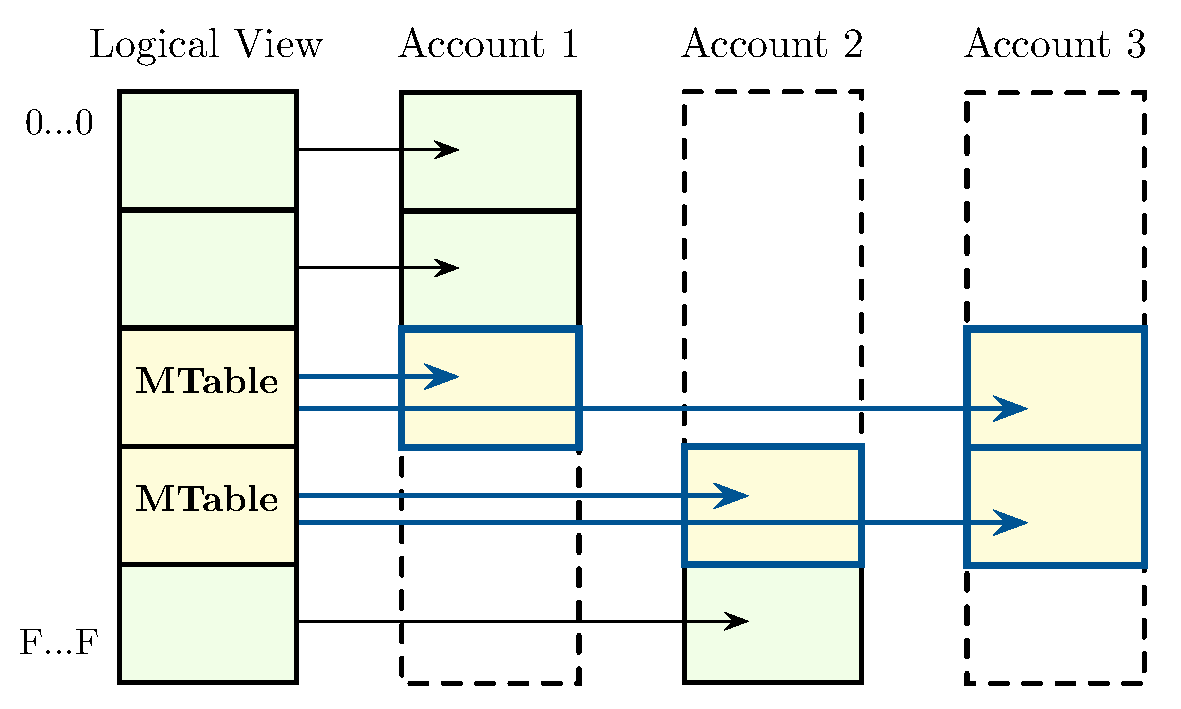
\includegraphics[width=\linewidth]{img/livemigration}
\caption{Resharding a data set when a third Azure storage account is added. Two key ranges are each migrated to the new account using a MigratingTable instance (abbreviated MTable).}
\label{fig:livemigration}
\end{figure}

% N.B. Artifact Services is mentioned at http://research.microsoft.com/en-us/people/schulte/.  Hopefully it's OK to reveal that it was the system in this case study. ~ Matt 2015-08-17
The initial motivation for MigratingTable was to solve a scaling problem for Artifact Services, an internal Microsoft system with a data set that is sharded across tables in different Azure storage accounts because it exceeds the limit on traffic supported by a single Azure storage account.  As the traffic continues to grow over time, the system needs to reshard the data set across a greater number of Azure storage accounts without interrupting service.  During such a resharding, our sharding manager will identify each key range that should migrate to a different table, and we will use a separate MigratingTable instance for each such key range to actually perform the migration (Figure~\ref{fig:livemigration}).  MigratingTable may also be useful to migrate data to a table with different values of configuration parameters that Azure does not support changing on an existing table, such as geographic location.

\def\term#1{\emph{#1}}
We also used \psharp to test the MigratingTable library, which is capable of transparently migrating a data set between tables in the Windows Azure storage service while an application is accessing the data set.

\begin{figure}[t]
\centering
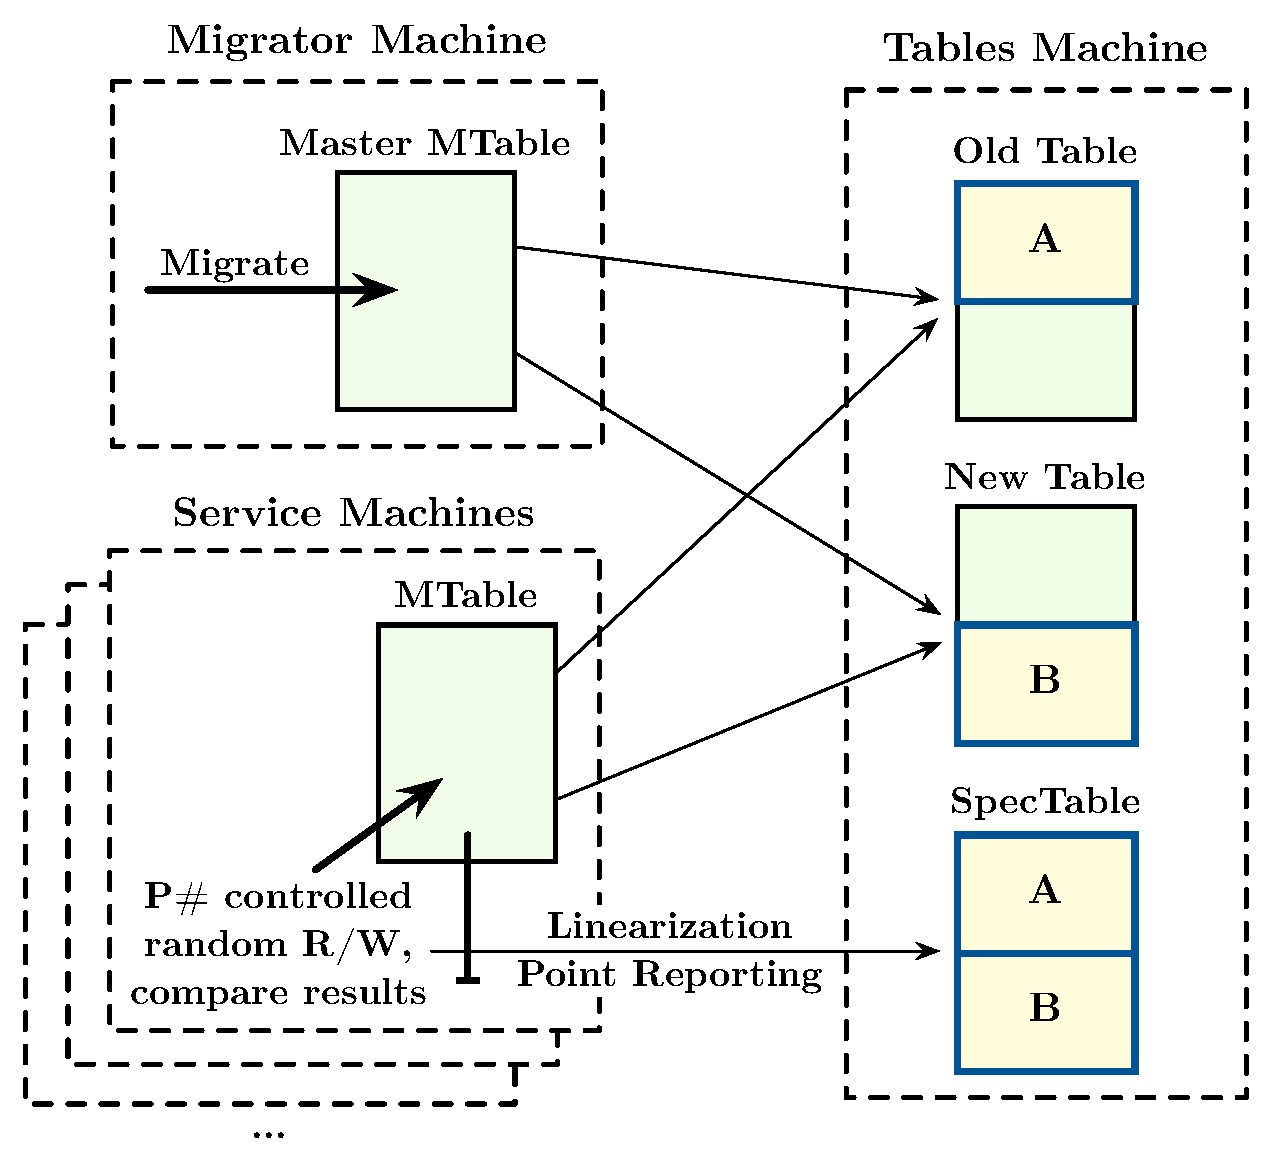
\includegraphics[width=\linewidth]{img/mocked_migration}
\caption{MigratingTable \psharp correctness test environment.}
\label{fig:mockedmigration}
\end{figure}

Since we were designing a new concurrent protocol that we expected to become increasingly complex over time as we add optimizations, we planned from the beginning to maintain a \psharp test harness along with the protocol to maintain confidence in its correctness.

MigratingTable implements an interface called IChainTable2, which provides the core read and write functionality of the original Azure table API with one exception: it provides \term{streaming reads} with a weaker consistency property than multi-page reads in the original API, since the original property would have been difficult to achieve for no benefit to applications we could foresee.  MigratingTable requires that its backend tables also implement IChainTable2, and we wrote a simple adapter to expose physical Azure tables as IChainTable2.  Our goal was then to verify that when multiple application processes issue ``input'' read and write calls to their own MigratingTable instances with the same backend tables, the behavior complies with the specification of IChainTable2 for the combined input history.

\subsubsection{Input generation}

Of course, there are many possible input histories to test.  Since we originally hoped for a comprehensive form of verification and we didn't feel we had good intuition to prepare a set of specific test cases that would make us confident of having caught any and all concurrency bugs in the protocol, it was natural for us to sample from a distribution of input histories that we defined to exercise all the features of IChainTable2 within certain bounds.  Furthermore, it was natural to let \psharp control the choice of input history as well as the machine interleaving so we could reproduce both using a single random seed.

All of our input histories include two application processes.  Each process performs either a single streaming read or a sequence of two atomic calls, each a read or a batch write.  Each batch write call includes one or two operations, where the operation type is chosen from the set supported by IChainTable2 (Insert, Replace, Merge, Delete, InsertOrReplace, InsertOrMerge, DeleteIfExists) and the row key is chosen from $\{0, \ldots, 5\}$.  If the operation requires an If-Match value, it is equally likely to be \texttt{*}, the current ETag of the row (if it exists), or some non-matching value.  Finally, the new entity includes a user-defined property \texttt{isHappy} whose value is equally likely to be true or false.  For both atomic and streaming reads, the filter expression is equally likely to be empty (i.e., match everything), \texttt{isHappy eq true}, or \texttt{isHappy eq false}.

\subsubsection{Model structure}

% N.B. SpecTable = InMemoryTableWithHistory in the current codebase. ~ Matt 2015-08-17
To comprehensively verify the behavior of MigratingTable under an arbitrary input history, we needed some formulation of the IChainTable2 specification to which to compare it.  Since the specification is deterministic under sequential calls except for the results of streaming reads, we decided the easiest approach was to write an in-memory reference implementation called SpecTable.  Given a streaming read call, SpecTable can produce a set of all results that are compliant with the specification.  Our correctness property is then:
% Convert to some theorem-like environment? ~ Matt
\begin{quote}
For every execution trace of a collection of MigratingTables backed by the same pair of \term{old} and \term{new} SpecTables (where \psharp chooses the actual result of each streaming read from the valid set) in parallel with the migrator job, there exists a linearization of the combined input history such that the output in the original trace matches the output of a ``reference'' SpecTable on the linearized input.
\end{quote}
%
We instrumented MigratingTable to report the intended \term{linearization point} of each input call, which in our setting is always one of the corresponding \term{backend calls} to the backend tables (often the last).  Specifically, after each backend call completes, MigratingTable reports whether that call was the linearization point, which may depend on the result of the call.  This makes it possible to verify the correctness property as the model executes.  The model consists of a \psharp \term{tables machine} containing all three SpecTables; a collection of \term{service machines} containing identically configured MigratingTables; and a \term{migrator machine} that performs the background migration (Figure~\ref{fig:mockedmigration}).  Each service machine issues a random sequence of input calls to its MigratingTable, which sends backend calls to the tables machine.  When MigratingTable reports the linearization point of an input call, the service machine sends that input call to the reference table.  When an input call completes, the service machine checks that the results from the MigratingTable and the reference table agree.  \psharp controls the interleaving of the backend calls.  To ensure that the reference table is never observed to be out of sync with the backend tables, after the tables machine processes a backend call, it enters a state that defers further backend calls until MigratingTable has reported whether the backend call was a linearization point and (if so) the call to the reference table has been made.  We use the \psharp random scheduling strategy; we were afraid that an exhaustive strategy would only be feasible within bounds so low that we would miss some bugs.

We wanted to implement the core MigratingTable algorithms in \csharp ``async/await'' code, like most of Artifact Services, to achieve both good readability and good performance.  We used a method similar to that described in Section~\ref{sec:psharp:async} to bring the generated TPL tasks under the control of the \psharp scheduler.  Then we implemented an ``async'' RPC mechanism based on the .NET RealProxy class that automates the generation of proxies for objects hosted by other \psharp machines (in our setting, the service machines use proxies for the SpecTables and various auxiliary objects hosted by the tables machine).  When a machine calls a method on a proxy, the proxy sends a \psharp message to the host machine, causing it to execute the method call on the original object and send back the result, which the proxy then returns.  Thus, the use of these proxies as IChainTable2 backends is transparent to the MigratingTable library, thanks to dynamic dispatch.

\subsection{An example bug in MigratingTable}
\MMComment{Move wherever appropriate}

One of the bugs in MigratingTable that we found using the \psharp test stands out because it reflects the type of oversight that tends to occur as designs evolve and it's unclear whether we would have been able to find it by any other method (\MMComment{revise remark when we have stress test results?}).  This bug, which we named QueryStreamedBackUpNewStream, is in the implementation of a streaming read from the virtual table, which should return a stream of all rows in the table sorted by key.  The essential implementation idea is to start streams $s_O$, $s_N$ from the old and new backend tables and merge the sorted streams by keeping track of the next row in each stream and returning the row with the lesser key.  In parallel, the migrator job is concurrently copying rows from the old table to the new table; we had satisfied ourselves that this concurrency would not cause any problems.  However, then we added support to the migrator job to delete the old table when it finishes copying, which triggers the virtual stream to close $s_O$.  Suppose the virtual stream is in a state in which the next row in $s_O$ has key $k_O$ and the next row in $s_N$ has key $k_N$, where $k_O < k_N$.  Further suppose that before the next read from the virtual stream, the migrator job copies a row with key $k$ ($k_O < k < k_N$) from the old table to the new table and then deletes the old table.  Since $s_O$ has not yet returned this row when it is closed and $s_N$ has already advanced to $k_N$, the row with key $k$ will be missed by the virtual stream.  A similar problem can occur if $s_N$ does not reflect rows inserted into the new table by the migrator job after $s_N$ is started, as allowed by the IChainTable2 specification.  Restarting $s_N$ when the old table is deleted fixes both variants of the bug.

\MMComment{Add a figure based on migration-bug3-explanation.pptx (probably a hybrid of slides 4 and 5, assuming we want only one figure).}

\subsection{Azure Service Fabric (change to CScale?)}
\label{sec:cases:fabric}

\PDComment{I guess we should write stuff about CScale here based on our last discussion: overview of the system (collection of Fabric services connected via TPL dataflow?), of its environment (Fabric), how they interop?, why its very challenging to test? how they test currently? I am not sure if all these should go here or be split here and the experience report, we will see ... same for the above case studies}

\emph{Azure Service Faric} (or \emph{Fabric} for short) is a platform and API for creating reliable services that execute on a cluster of machines. The developer writes a service that receives requests (e.g.\ from some client program via HTTP requests) and mutates its state based on these requests. In order to make the service \emph{reliable}, Fabric launches several copies (\emph{replicas}) of the service, where each copy runs as a separate process on a different node in the cluster. One replica is selected to be the \emph{primary} which serves client requests; the rest are \emph{secondaries}. The primary replicates state changes to the secondaries by sending \emph{replication requests} so that all replicas eventually have the same state. If the primary fails (e.g.\ if the node on which the primary is running crashes), Fabric elects one of the secondaries to be the new primary and launches another secondary; the new secondary will receive a full or partial copy (depending on whether persistent storage is used) of the state of the new primary in order to ``catch up'' with the other secondaries. Fabric provides a name-resolution service so that clients can always find the current primary. 

Fabric services have a lot of asynchrony, which make them interesting targets for systematic testing with \psharp{}.
Our primary goal was to create a \psharp{} model of Fabric to allow
thorough testing of services, where Fabric's asynchrony is controlled 
by the \psharp{} runtime.
The system that we wished to test is \emph{CScale}~\cite{X},
a big data-stream processing system that chains multiple Fabric services
in a directed acyclic graph.
Prior work~\cite{deligiannis2015psharp}
created a model of Fabric with limited functionality;
it used a mixture of \csharp{} and \psharp{} internally,
only supported one in-flight replication request
(which restricts the asynchrony that can be tested),
and only supported one Fabric service.
Our new Fabric model was re-written to use only \psharp{}
internally,
support an arbitrary number of Fabric services and in-flight replication requests,
and in general be a more complete model of Fabric.
Note that \csharp{} code is still required to interface with the existing
\csharp{} service code.
We refer to our \csharp{} code
as the \emph{translation layer}
and
 the user-written \csharp{} service code as \emph{user code}. 

\begin{figure}[thb]
\centering
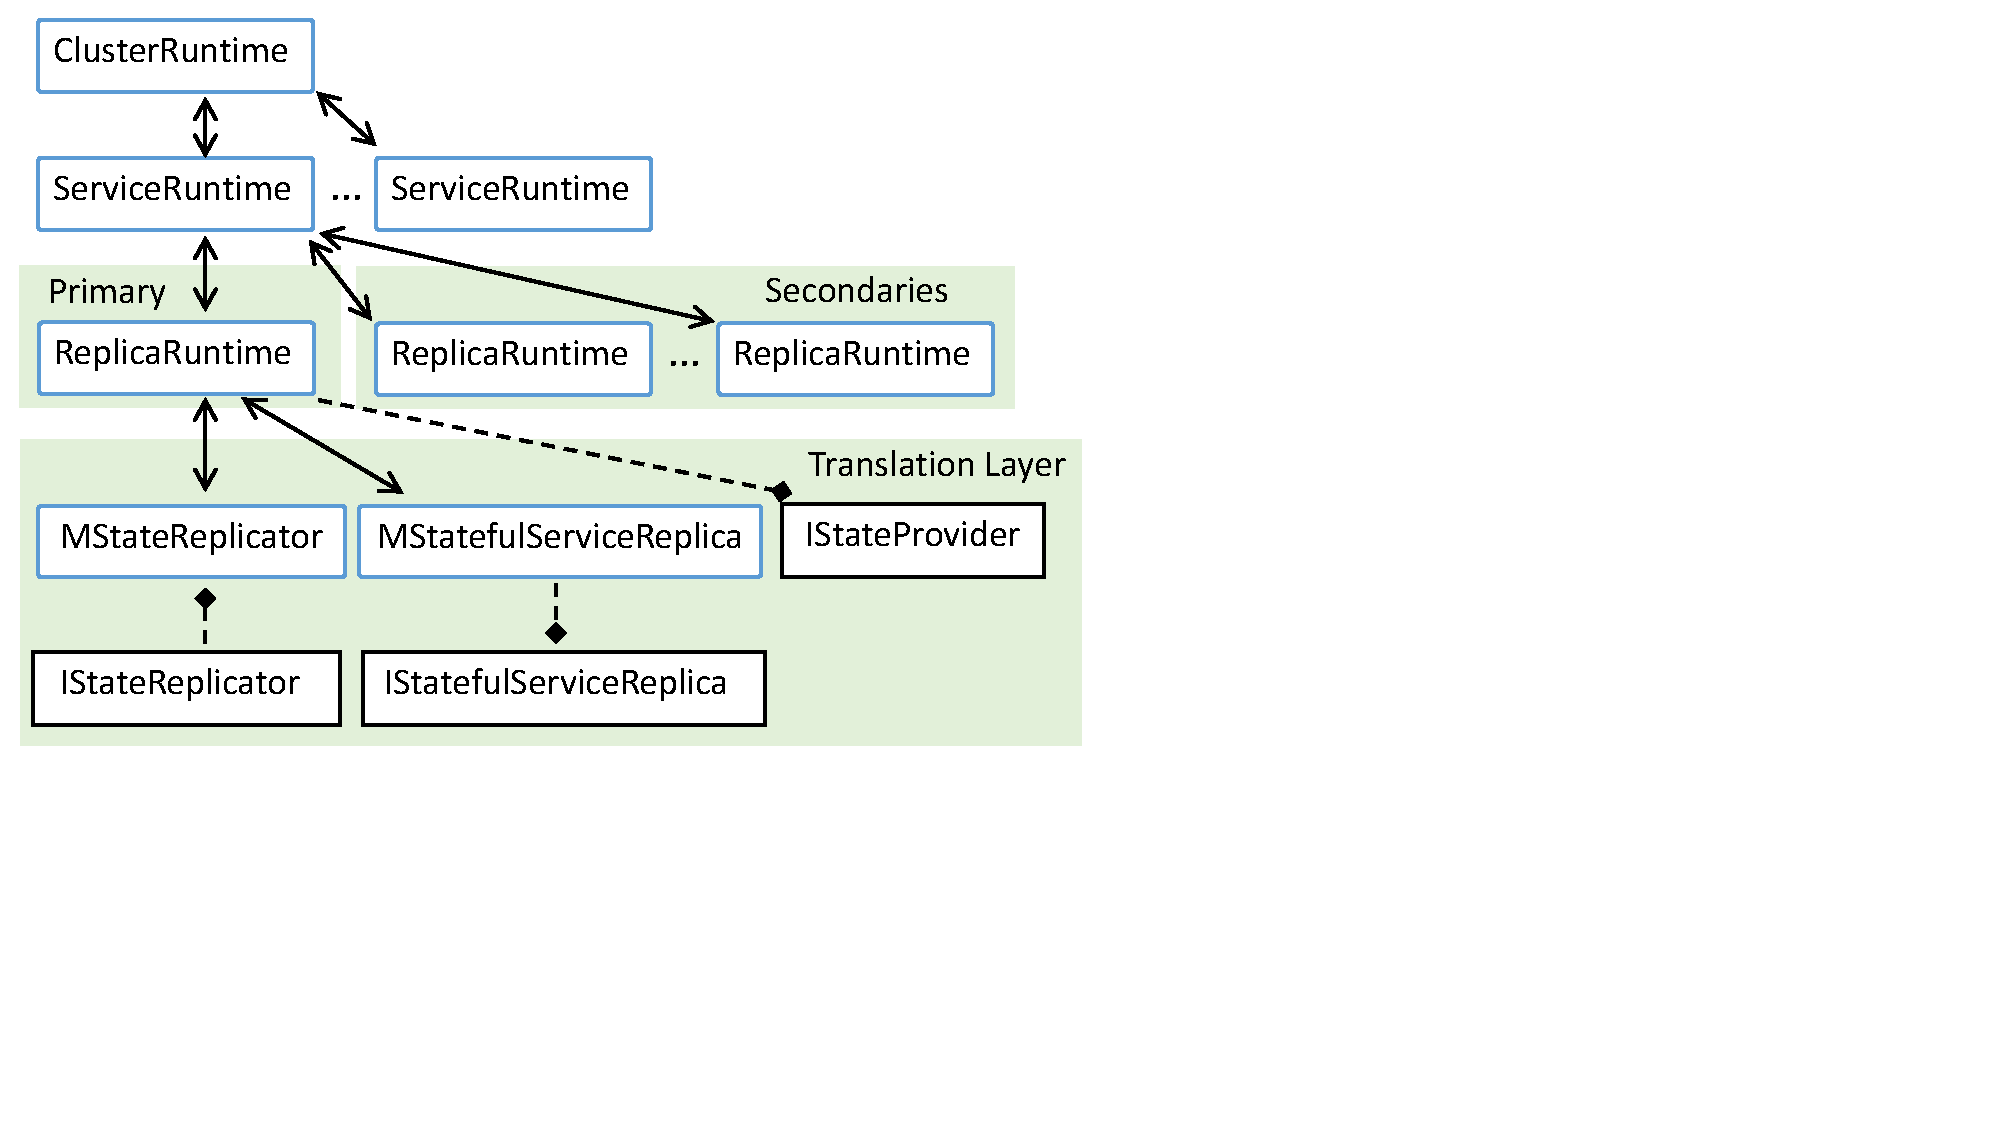
\includegraphics[width=\linewidth, clip=true, trim=0 180px 440px 0]{img/FabricModelOverview}
\caption{Overview of the key machines (rounded boxes) and interfaces (boxes) in our Fabric model.}
\label{fig:fabric_model}
\end{figure}

An overview of our Fabric model is shown in Figure~\ref{fig:fabric_model}.
The \texttt{ClusterRuntime} machine 
handles the creation and management of 
one or more Fabric services,
as well as service resolution requests
which allows for client-service and inter-service communication
within the model.
Each Fabric service instance is managed by a \texttt{ServiceRuntime}
machine, which in turn manages 
several \texttt{ReplicaRuntime} machines.
Each \texttt{ReplicaRuntime} communicates with the user code
via several machines and interfaces from the translation layer
(only the translation layer for the primary is shown,
but every \texttt{ReplicaRuntime} has its own instance of the translation layer).
Note that communication between machines is hierachical;
thus, communication between \texttt{ReplicaRuntime}s
(such as the sending of replication requests)
is via the \texttt{ServiceRuntime} machine for that service.
This approach does not necessarily reflect how Fabric works in practice.
Instead, we chose an architecture
that keeps the model simple
while still allowing (what we believe to be) realistic
asynchrony and failure scenarios.
 

